\section{Bidirectional Cross}
\textit{An elementary topology where network coding can provide interesting benefits is the bidirectional cross, where we distinguish between three cases:}\\

\begin{figure}[!h]
  \centering
  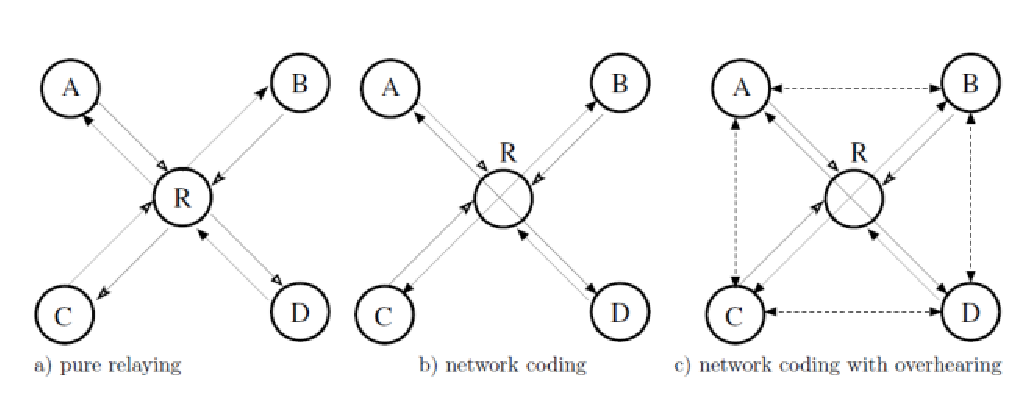
\includegraphics[width=15cm]{Bidirectional_Cross.eps}
  \caption{Bidirectional Cross}
  \label{fig:Bidirectional_Cross}
\end{figure}

\textit{Specifically, the cases are (a) pure relaying, where packets are not combined, (b) network coding, where two packets are combined, and (c) network coding with overhearing, where the relay combines four packets.}


\subsection{Exercise 3: Activities.}
\textit{Give the activities for each node in the topology for cases (a), (b), and (c). The possible activities for each node are idle, receive, and send. The following tables are intended as a help to construct the respective activity plots.}\\

Something...

\subsection{Exercise 2: Throughput With Network Coding}
\textit{Repeat the steps of the previous question but using inter-session network coding at the relay. How many regions of operations are there and why?}

\subsubsection{(a) Pure Relaying}
\begin{figure}[!h]
  \centering
  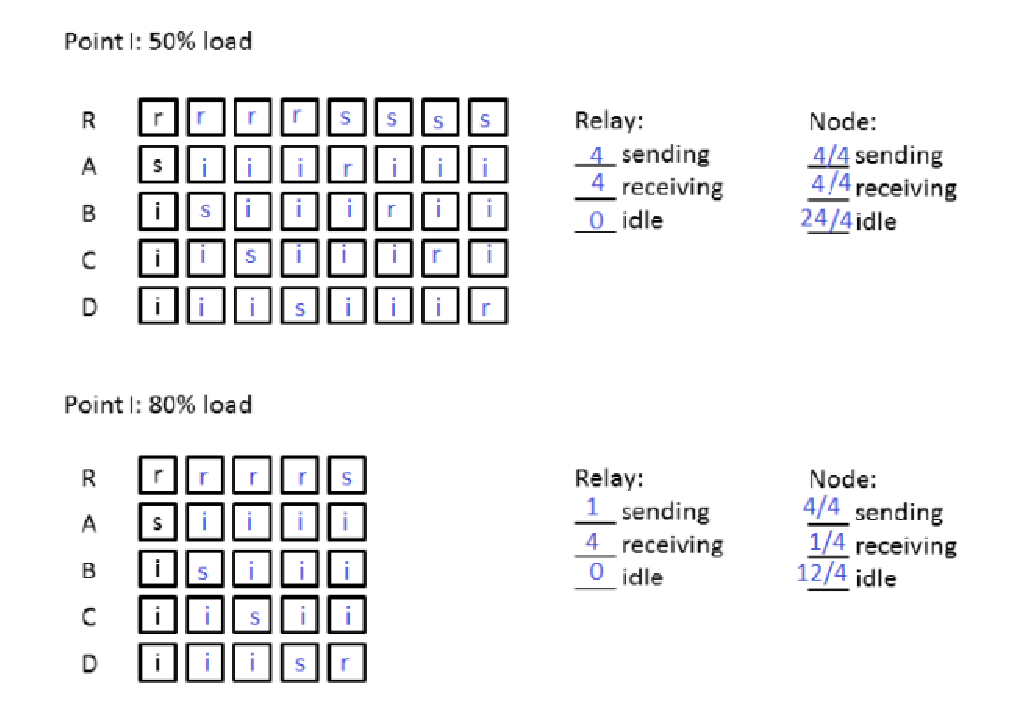
\includegraphics[width=15cm]{Pure_relaying.eps}
  \caption{Pure Relaying}
  \label{fig:Pure_relaying}
\end{figure}
\newpage
\subsubsection{(b) Network Coding}
\begin{figure}[!h]
  \centering
  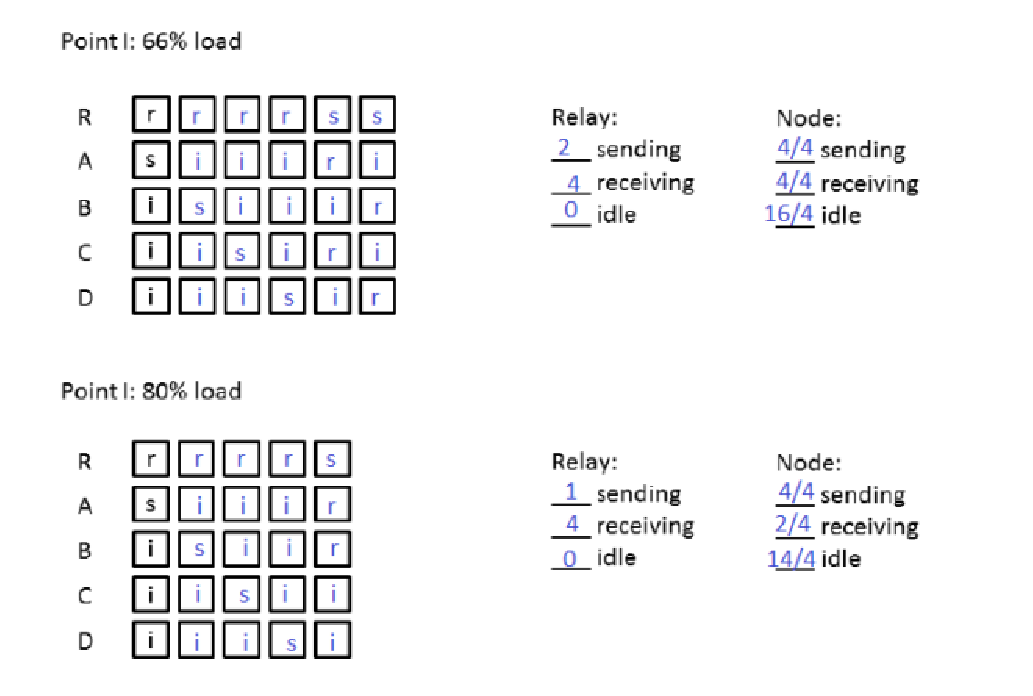
\includegraphics[width=15cm]{network_coding.eps}
  \caption{Network Coding}
  \label{fig:network_coding}
\end{figure}
\newpage
\subsubsection{(c) Network Coding with Overhearing}
\begin{figure}[!h]
  \centering
  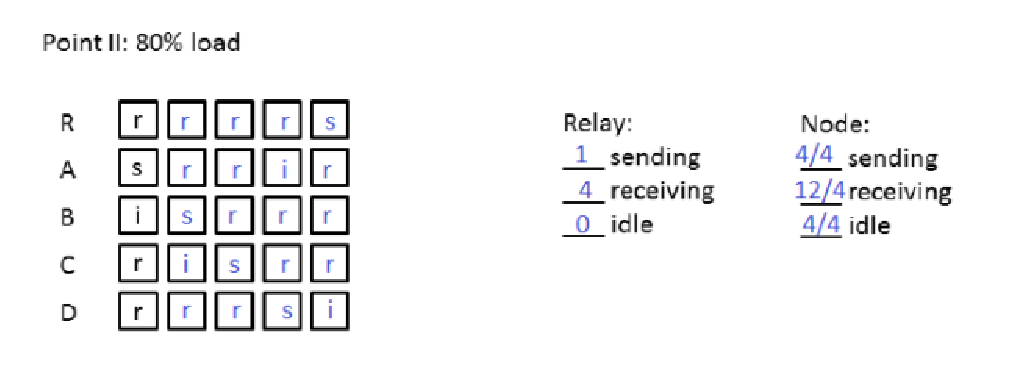
\includegraphics[width=15cm]{network_coding_overhearing.eps}
  \caption{Network Coding Overhearing}
  \label{fig:network_coding_overhearing}
\end{figure}

\subsection{Exercise 4: Throughput}
\textit{Give the total throughput for the three cases (a), (b), and (c), including the plot and the analytical expressions}\\

Something...